% IEEE conference paper. Every number, table and figure comes from scripts/paper_build.py:
% this file contains none of its own (tests/test_paper.py enforces that).
% Build the inputs:   python scripts/paper_build.py --figures
% Compile:            pdflatex main && bibtex main && pdflatex main && pdflatex main
% (IEEEtran.cls is on Overleaf and in every TeX distribution; this repository does not ship it.)
\documentclass[conference]{IEEEtran}
\IEEEoverridecommandlockouts
\usepackage{cite}
\usepackage{amsmath,amssymb,amsfonts}
\usepackage{graphicx}
\usepackage{textcomp}
\usepackage{xcolor}
\usepackage{url}

% Generated by scripts/paper_build.py from data/cea/*.csv. Do not edit by hand.
\newcommand{\avgHigh}{0.8226}
\newcommand{\avgLow}{0.6751}
\newcommand{\bandHigh}{0.7400}
\newcommand{\bandLow}{0.6874}
\newcommand{\bandOutside}{outside}
\newcommand{\bandPublished}{0.6751}
\newcommand{\baseYear}{2023-24}
\newcommand{\covEighty}{10}
\newcommand{\covEightyOf}{12}
\newcommand{\covNinety}{11}
\newcommand{\covNinetyOf}{12}
\newcommand{\dAfter}{7.20}
\newcommand{\dDeadline}{2.45}
\newcommand{\dateFirst}{November 2006}
\newcommand{\dateLast}{August 2026}
\newcommand{\deadline}{31 July 2026}
\newcommand{\effectLatest}{4.87}
\newcommand{\effectRevision}{0.78}
\newcommand{\effectSeries}{21.85}
\newcommand{\fAfter}{0.6751}
\newcommand{\fBase}{0.7275}
\newcommand{\fDeadline}{0.7097}
\newcommand{\firstFY}{2000-01}
\newcommand{\fyAssess}{2025-26}
\newcommand{\fyAtDeadline}{2024-25}
\newcommand{\gapReadings}{4.87}
\newcommand{\lastFY}{2025-26}
\newcommand{\lastStated}{1 August 2026}
\newcommand{\lastStep}{1.52}
\newcommand{\lastStepFY}{2025-26}
\newcommand{\lastVersion}{22}
\newcommand{\lvlHigh}{90}
\newcommand{\lvlLow}{80}
\newcommand{\maxRev}{0.96}
\newcommand{\maxStep}{6.01}
\newcommand{\medRev}{0.07}
\newcommand{\medStep}{1.25}
\newcommand{\nBeating}{0}
\newcommand{\nIndia}{884}
\newcommand{\nModels}{4}
\newcommand{\nOverOne}{18}
\newcommand{\nOverThree}{4}
\newcommand{\nSeriesKeys}{11}
\newcommand{\nSteps}{25}
\newcommand{\nTargets}{20}
\newcommand{\nValues}{2,071}
\newcommand{\nVersions}{23}
\newcommand{\nYears}{26}
\newcommand{\naiveMAE}{1.99}
\newcommand{\naiveRMSE}{2.41}
\newcommand{\naiveWorst}{5.70}
\newcommand{\revLargestFY}{2020-21}
\newcommand{\shNeeded1After}{14}
\newcommand{\shNeeded1Deadline}{41}
\newcommand{\shNeeded3After}{42}
\newcommand{\shaFactors}{3e4976f355c5}
\newcommand{\shaVersions}{4fc73f81ffef}
\newcommand{\shareSeries}{23}
\newcommand{\spreadTwoOne}{17.5}
\newcommand{\spreadTwoTwo}{21.85}
\newcommand{\tgtHigh}{3}
\newcommand{\tgtLow}{1}
\newcommand{\thresh}{5}
\newcommand{\uploadFolder}{2026/09}
\newcommand{\verAfter}{22}
\newcommand{\verDeadline}{21}
\newcommand{\yearFirst}{2006}
\newcommand{\yearLast}{2026}

% An open item. python scripts/paper_build.py --submit-check lists every one still in the text.
\newcommand{\verify}[1]{\textcolor{red}{\textbf{[VERIFY: #1]}}}
\newcommand{\tCO}{t\,CO\textsubscript{2}}

\begin{document}

\title{One Rule, Several Numbers: Version and Series Ambiguity in the Grid Emission Factor of India's Carbon Credit Trading Scheme}

\author{\IEEEauthorblockN{\verify{authors, in order}}
\IEEEauthorblockA{RV College of Engineering, Bengaluru, India\\
\verify{emails and ORCID iDs}}}

\maketitle

\begin{abstract}
India's Carbon Credit Trading Scheme sets emission-intensity targets for industrial plants, and its compliance procedure directs plants to use ``the latest average grid emission factor'' published by the Central Electricity Authority (CEA). Using a machine-readable record of all \nVersions{} versions of the CEA CO\textsubscript{2} Baseline Database (\dateFirst{} to \dateLast{}), we show that this rule does not select one number. The factor for FY\fyAssess{} first appears in a version dated \lastStated{}, after the \deadline{} reporting deadline. The two readings of ``latest'' differ by \gapReadings{}\%, and CEA's four all-India average series for that year span \spreadTwoTwo{}\%. A plant whose target basis has a Scope~2 share $s$ sees its reported intensity change by $s$ times these percentages with no change in operations. Year-on-year steps in the factor exceed \tgtLow{}\% in \nOverOne{} of \nSteps{} years, last year's value misses the next by \naiveMAE{}\% on average, and none of \nModels{} alternative models has a lower mean error. All numbers, tables and figures are generated from the open registry by one script.
\end{abstract}

\begin{IEEEkeywords}
grid emission factor, carbon market, India, emission intensity, version history, reproducibility
\end{IEEEkeywords}

\section{Introduction}
Calculating the emissions from purchased electricity is multiplication: electricity consumed times a grid emission factor. Showing that the figure is the right one is harder, because it depends on which factor, and which version of it, was used. In India the reference factors are published by the Central Electricity Authority (CEA) in its CO\textsubscript{2} Baseline Database~\cite{cea}, reissued about once a year with earlier years restated.

India's Carbon Credit Trading Scheme (CCTS) sets targets for the greenhouse gas emission intensity (GEI) of plants in notified sectors, in tonnes of CO\textsubscript{2}-equivalent per unit of product, covering Scope~1 and Scope~2 emissions gate to gate. The FY\fyAssess{} targets ask for a reduction of \tgtLow{} to \tgtHigh{}\%~\verify{cite the target notification}. The compliance procedure of the Bureau of Energy Efficiency (BEE)~\cite{bee} says that emissions from electricity ``shall be calculated by considering the latest average grid emission factors from CO2 baseline database for Indian Power Sector''~\verify{quotation is from one PDF whose internal date precedes the reported notification; confirm against the notified text}.

That revisions to emission factors matter is not new: the GHG Protocol requires a base year to be recalculated when emission factors are updated~\cite{ghg,scope2}, and the Science Based Targets initiative treats a change of \thresh{}\% or more as significant~\cite{sbti}\verify{confirm the threshold and its wording}. Our point is narrower. A compliance rule that names ``the latest average'' factor admits several readings, and the readings give different numbers for the same plant. We make three contributions.
\begin{itemize}
\item A record of every factor in every published CEA version, with its workbook cell and a file checksum (Section~\ref{sec:data}).
\item A measurement of how far apart the readings of the rule are, expressed as a change in a plant's reported intensity per unit of Scope~2 share (Sections~\ref{sec:readings} and~\ref{sec:materiality}).
\item A measurement of how large year-on-year factor changes are, and how well the missing year can be predicted (Sections~\ref{sec:steps} and~\ref{sec:nowcast}).
\end{itemize}
Every percentage in this paper that refers to intensity applies to the Scope~2 share of a plant's target basis, not to its total.

\section{Data and Method}\label{sec:data}
\subsection{The registry}
CEA's database page lists \nVersions{} versions, with stated dates from \dateFirst{} to \dateLast{}. We downloaded every workbook and user guide, recorded each file's address and SHA-256 checksum, and read the \texttt{Results} sheet of each with one parser that handles the three layouts found. Every row label is mapped explicitly to one of \nSeriesKeys{} factor series, and an unmapped label stops the run. The registry holds \nValues{} values for financial years \firstFY{} to \lastFY{} (\nYears{} years), of which \nIndia{} are all-India; the rest are regional values published in early versions. Values are stored as found in the workbook, at full precision and unadjusted. Each is linked to its sheet and cell and to CEA's own row label. A version's date is the date written in its workbook; for some versions only a month is given. The registry is open~\cite{repo}.

\subsection{Definitions}
Let $f_{v}(y)$ be the value of one series for financial year $y$ in version $v$. A \emph{step} is the first-published year-on-year change: $f_v(y)$ against $f_v(y-1)$ in the version $v$ that first published $y$. A \emph{revision} is the change in a year's value between the first version that published it and the latest. Steps that CEA flags as a change of method are excluded. For a plant with fixed fuel use, electricity use and production, let $s$ be the share of its baseline-year emissions, in the target basis, that comes from purchased electricity. Replacing the baseline factor $f_b$ by an assessment factor $f_a$ changes its intensity by exactly
\begin{equation}
\frac{\Delta\mathrm{GEI}}{\mathrm{GEI}_b} = s\left(\frac{f_a}{f_b}-1\right),
\label{eq:gei}
\end{equation}
since $\mathrm{GEI}=(C+E f)/P$ for combustion emissions $C$, electricity $E$ and production $P$, and $s = E f_b/(C+E f_b)$. This is arithmetic, not a model; it uses no plant data.

\subsection{Predicting the missing year}
To ask how well a year's factor can be predicted before CEA publishes it, each year's first-published value is the target, and each forecast uses only values from versions published before that one (no look-ahead). We compare last year's value (naive), drift, recent drift, a linear trend and an AR(1) model on changes~\cite{hyndman}. Bands are built from the quantiles of earlier naive errors, and their coverage is measured out of sample.

\section{What the Rule Allows}\label{sec:readings}
The procedure leaves three things open: \emph{latest as of when} (the end of the year, the reporting date, or the date of verification), \emph{which average} (CEA publishes several), and consistency with the baseline. Elsewhere it requires that factors be ``consistently applied for baseline and assessment year''~\verify{this sentence is in a paragraph about fuel and material factors; confirm whether it covers the grid factor}. This gives three readings.

\emph{Timing.} The first version that covers FY\fyAssess{}, version~\verAfter{}, is dated \lastStated{} in its own workbook, one day after the \deadline{} deadline, and its download address sits under CEA's \uploadFolder{} upload folder. At the deadline, the newest published factor was for FY\fyAtDeadline{}, in version~\verDeadline{}: \fDeadline{}~\tCO{}/MWh. Once version~\verAfter{} appeared, the newest was \fAfter{}, which is \gapReadings{}\% lower. Both are ``the latest''.

\emph{Series.} For FY\fyAssess{}, the four all-India average series in version~\verAfter{} range from \avgLow{} to \avgHigh{}~\tCO{}/MWh, a spread of \spreadTwoTwo{}\% (\spreadTwoOne{}\% for FY\fyAtDeadline{} in version~\verDeadline{}). The procedure does not name one. Fig.~\ref{fig:candidates} shows the candidates a verifier could pick.

\begin{figure}[t]
\centering
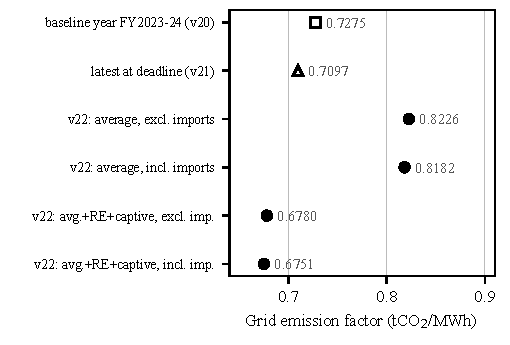
\includegraphics[width=\columnwidth]{figs/fig_candidates.pdf}
\caption{Candidate grid emission factors for assessing FY\fyAssess{}: the baseline-year factor, the latest factor at the reporting deadline, and the four all-India average series in version~\verAfter{}. The first two values are for the series that includes renewable and captive generation and imports.}
\label{fig:candidates}
\end{figure}

Table~\ref{tab:readings} applies Eq.~\eqref{eq:gei} to the all-India series that includes renewable and captive generation and imports (one of the four in Fig.~\ref{fig:candidates}), with FY\baseYear{} as the baseline year\verify{BEE's procedure does not name a baseline year; FY\baseYear{} is assumed}. Under the baseline-year reading the factor contributes nothing. Under the deadline reading a plant with a Scope~2 share of \shNeeded1Deadline{}\% shows a \tgtLow{}\% reduction without changing anything; under the post-publication reading, \shNeeded1After{}\%, and a share of \shNeeded3After{}\% shows the full \tgtHigh{}\%.

\begin{table}[t]
\caption{Intensity reduction shown with no physical change, by reading of the rule, and the Scope~2 share $s$ that shows the lower and upper target.}
\label{tab:readings}
\centering
\footnotesize
\begin{tabular}{@{}p{2.1cm}rrrrr@{}}
\hline
Reading & Factor & Ver. & Change & $s$ for low & $s$ for high \\
\hline
% Generated by scripts/paper_build.py. Do not edit by hand.
Same factor as the baseline year & 0.7275 & v20 & 0.00\% & never & never \\
Latest at the reporting deadline & 0.7097 & v21 & $-$2.45\% & 41\% & never \\
Latest once the FY2025-26 factor exists & 0.6751 & v22 & $-$7.20\% & 14\% & 42\% \\

\hline
\end{tabular}
\end{table}

\section{Materiality}\label{sec:materiality}
By Eq.~\eqref{eq:gei}, a factor change of $d$ percent moves a total by $s\,d$ percent. Fig.~\ref{fig:sensitivity} plots this for three kinds of change: the choice of series (\effectSeries{}\%), the reading of ``latest'' (\effectLatest{}\%) and the revision of a past year by CEA (at most \effectRevision{}\%, for FY\revLargestFY{}, in the series with renewable and captive generation). The series choice alone moves a total by more than the \thresh{}\% threshold once the Scope~2 share exceeds \shareSeries{}\%; neither the reading of ``latest'' nor a revision reaches it at any share. If the targets count only combustion and electricity emissions and not process emissions~\verify{BEE's note on process emissions; confirm}, the relevant $s$ is the share within that basis, which is larger than the share within a full inventory in sectors with large process emissions, such as cement, iron and steel and refining. We have not measured $s$ for any sector.

\begin{figure}[t]
\centering
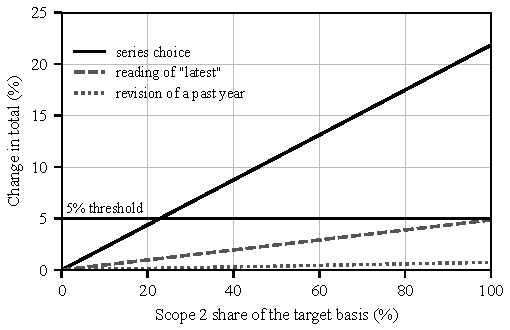
\includegraphics[width=\columnwidth]{figs/fig_sensitivity.pdf}
\caption{Change in a plant's total from a grid-factor change alone, against the Scope~2 share of its target basis. Lines are straight by Eq.~\eqref{eq:gei}.}
\label{fig:sensitivity}
\end{figure}

\section{How Large Are Year-on-Year Changes?}\label{sec:steps}
For the weighted average including imports, the longest all-India series, \nOverOne{} of \nSteps{} first-published steps exceed \tgtLow{}\% and \nOverThree{} exceed \tgtHigh{}\% (median \medStep{}\%, maximum \maxStep{}\%; Fig.~\ref{fig:steps}). The steps are of the same size as the targets, but they matter for intensity only through $s$. Once published, a year is restated by a median of \medRev{}\% and at most \maxRev{}\%: which year's factor is used matters more than which version of it. Table~\ref{tab:steps} repeats the summary for the long all-India series.

\begin{figure}[t]
\centering
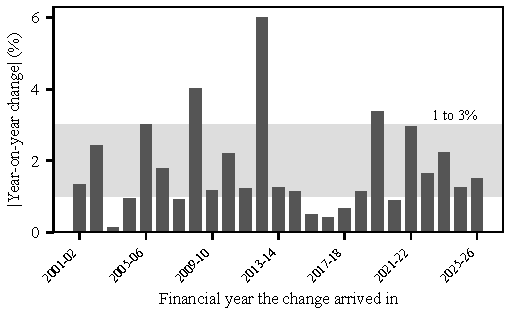
\includegraphics[width=\columnwidth]{figs/fig_steps.pdf}
\caption{Size of each first-published year-on-year change in the weighted average including imports. The shaded band is the target range.}
\label{fig:steps}
\end{figure}

\begin{table}[t]
\caption{First-published year-on-year steps and revisions, all-India series with at least twenty steps.}
\label{tab:steps}
\centering
\footnotesize
\begin{tabular}{@{}p{2.6cm}rrrrrr@{}}
\hline
Series & Steps & Median & Max & $>$low & $>$high & Rev. \\
\hline
% Generated by scripts/paper_build.py. Do not edit by hand.
Weighted average, excl. imports & 25 & 1.28\% & 5.98\% & 17 & 4 & 0.04\% \\
Weighted average, incl. imports & 25 & 1.25\% & 6.01\% & 18 & 4 & 0.07\% \\
Operating margin, excl. imports & 25 & 0.86\% & 3.09\% & 7 & 1 & 0.04\% \\
Operating margin, incl. imports & 25 & 0.89\% & 3.09\% & 8 & 1 & 0.07\% \\
Combined margin, excl. imports & 24 & 1.14\% & 5.19\% & 13 & 5 & 0.07\% \\
Combined margin, incl. imports & 24 & 1.34\% & 5.85\% & 13 & 5 & 0.09\% \\
Build margin, excl. imports & 20 & 2.51\% & 13.35\% & 15 & 9 & 0.03\% \\

\hline
\end{tabular}
\end{table}

\section{Predicting the Missing Year}\label{sec:nowcast}
Over \nTargets{} years of the weighted average including imports, using last year's value as the forecast misses the new value by \naiveMAE{}\% on average (RMSE \naiveRMSE{}\%, worst \naiveWorst{}\%). None of the \nModels{} alternatives has a lower mean absolute error than the naive forecast (Table~\ref{tab:nowcast}); with this few years, a sign test on the years won can only detect a large difference. A band built from earlier errors contained \covEighty{} of \covEightyOf{} later values at the nominal \lvlLow{}\% level and \covNinety{} of \covNinetyOf{} at \lvlHigh{}\%. For the series with renewables and captive plants, the published FY\fyAssess{} value, \bandPublished{}, fell \bandOutside{} the \lvlHigh{}\% band, \bandLow{} to \bandHigh{}, drawn from earlier years.

\begin{table}[t]
\caption{One-year-ahead forecasts of the first-published value, mean absolute and root-mean-square error, years in which the model beats the naive forecast, and the sign-test $p$.}
\label{tab:nowcast}
\centering
\footnotesize
\begin{tabular}{@{}p{3.1cm}rrrr@{}}
\hline
Model & MAE & RMSE & Beats naive & $p$ \\
\hline
% Generated by scripts/paper_build.py. Do not edit by hand.
naive (last year's value) & 1.99\% & 2.41\% & -- & -- \\
drift (average change so far) & 2.04\% & 2.55\% & 7/20 & 0.26 \\
recent drift (last three changes) & 2.31\% & 3.00\% & 6/20 & 0.12 \\
linear trend & 2.84\% & 3.14\% & 7/20 & 0.26 \\
AR(1) on changes & 2.12\% & 2.67\% & 8/20 & 0.50 \\

\hline
\end{tabular}
\end{table}

\section{Discussion}
The rule could be made to give one number with four changes: name the series by its exact title; fix the vintage (for example, the factor for the compliance year as published in the first version that covers it, with a stated fallback if it is not out by the reporting date); require the report to state the version and series used, so that a verifier can reproduce the figure; and publish equivalence factors for multi-product plants, or require each entity's factors to be declared and verified. These are suggestions from the text alone~\verify{check later BEE guidance, FAQs and target notifications; if any already settle these points, the framing changes from ``the rule is open'' to ``the procedure left this open and it was later settled by X''}.

\section{Limitations}
(i)~The procedure was read from one document whose internal date precedes the reported notification; every quotation must be confirmed against the notified text. (ii)~The baseline year is assumed. (iii)~No plant, real or synthetic, enters any number, and no sector is placed on the curve, because we have no cited sector shares of the target basis. (iv)~We do not know what verifiers applied in the first cycle. (v)~The forecasting numbers rest on about twenty values of one series. (vi)~Version dates are the dates in the workbooks, not publication dates. (vii)~The data are compiled from CEA's workbooks, are not an official CEA product, and say nothing about any entity's compliance.

\section{Conclusion}
A rule that directs plants to ``the latest average grid emission factor'' does not determine one number: for the first compliance year the readings differ by \gapReadings{}\% in the factor and the series differ by \spreadTwoTwo{}\%, and a plant's reported intensity moves by its Scope~2 share times those amounts. Naming the series and the vintage in the procedure would remove the ambiguity.

\section*{Reproducibility}
All numbers in this paper are macros written by \texttt{scripts/paper\_build.py} from \texttt{data/cea/factors.csv} (SHA-256 \shaFactors{}\ldots) and \texttt{data/cea/versions.csv} (SHA-256 \shaVersions{}\ldots); the tables and figures are generated by the same script, and \texttt{python scripts/paper\_build.py --check} fails if any committed file differs from what the data give. The registry, scripts and tests are in the repository~\cite{repo}; the registry is to be deposited with a DOI\verify{Zenodo DOI, licence and CEA redistribution terms}.

\section*{Acknowledgment}
The data are compiled from publications of the Central Electricity Authority, Ministry of Power, Government of India. \verify{thanks and funding, or none} The software that produced the data and numbers, and drafts of this text, were developed with substantial assistance from an AI coding assistant (Claude, Anthropic); the authors reviewed the content and are responsible for it\verify{use the venue's required wording for AI-use disclosure; see docs/AI\_USE.md}.

\begin{thebibliography}{00}
\bibitem{cea} Central Electricity Authority, Ministry of Power, Government of India, ``CO\textsubscript{2} baseline database for the Indian power sector,'' \url{https://cea.nic.in/cdm-co2-baseline-database/} (files retrieved 26 September 2026).
\bibitem{bee} Bureau of Energy Efficiency, Ministry of Power, Government of India, ``Detailed procedure for compliance mechanism under the Carbon Credit Trading Scheme.'' \verify{exact title, version, date and notification reference}
\bibitem{ghg} World Resources Institute and World Business Council for Sustainable Development, \emph{The Greenhouse Gas Protocol: A Corporate Accounting and Reporting Standard}, rev. ed., 2004.
\bibitem{scope2} World Resources Institute, \emph{GHG Protocol Scope 2 Guidance: An Amendment to the GHG Protocol Corporate Standard}, 2015.
\bibitem{sbti} Science Based Targets initiative, ``SBTi criteria and recommendations.'' \verify{document title, version, year and URL}
\bibitem{hyndman} R.~J. Hyndman and G. Athanasopoulos, \emph{Forecasting: Principles and Practice}, 3rd ed. Melbourne: OTexts, 2021.
\bibitem{repo} ``CarbonX: open registry of India's CEA grid emission factors, with build scripts,'' \url{https://github.com/Shreyaskale7/CarbonX}. \verify{Zenodo DOI once minted}
\end{thebibliography}

\end{document}
